\begin{table}[ht]
    \caption{Ausgewählte Operationsverstärker-Grundschaltungen}
    \label{tab:Grundschaltungen}
    \begin{tabular}{|m{0.24\textwidth}|m{0.405\textwidth}|m{0.33\textwidth}|}
    \hline
    Schaltung & Frequenzgang und Gleichung & Erläuterung und Eigenschaften\\ % Neue Zeile mit Text
    \hline
    \vspace{0.5cm}
    \centering
    \begin{circuitikz}[scale=0.7, transform shape]
    \ctikzset{
         resistors/scale=0.8,              
         tripoles/en amp/height=1.4, % Höhe des OPV             
         tripoles/en amp/width=1.4,   % Breite des OPV
         tripoles/en amp/input height=-0.45
    }
    \vspace{1ex}
    \draw (2,-0.1) node[en amp] (opamp) {}
    (opamp.+) --++ (-0.5,0) node[ocirc, label=left:$U_E$] (eingang) {} 
    (opamp.out) --++ (0.5,0) node[ocirc, label=right:$U_A$] {}
    (opamp.-) -- ++(0, -1.5) to[R, l=$R_1$] ++(0, -1) node[ground] {}
    (opamp.out) node[circ] {} -- ++(0,-1.5) to[R, l=$R_2$] ++(-1.95,0) node[circ] (feedback) {};
\end{circuitikz}

 & \begin{tikzpicture}[scale=1, transform shape]
    \begin{axis}[
    width=4.5cm, % Breite des Graphen
    height=3.5cm, % Höhe des Graphen
    xmin=0, xmax=10,
    ymin=0, ymax=120,
    axis lines=left,
    axis on top=true,
    domain=0:10,
    xtick=\empty,
    ytick=\empty,
    ylabel style={rotate=270, anchor=east, yshift=1cm}, % Position der Beschriftung oben links, horizontal
     ylabel={\it V}, % Hier die gewünschte Beschriftung einfügen
    xlabel={f[Hz]},
    clip mode=individual % Verhindert das Abschneiden von Elementen
    ]
    \path[draw=none] (axis cs:-4, 0) rectangle (axis cs:16.6,120);
    
    
    \coordinate (xaxis) at (axis description cs:15.5,0); % Verwendet die relative Positionierung für x-Achse
    
    \addplot+[mark=none, thick, blue] coordinates {(0,80) (10,80)};
    % Adding the left-side label
    \node[anchor=east] at (axis cs:0,80) {$1 + \frac{R_2}{R_1}$};
    \end{axis}
    \begin{axis}[
    width=4.5cm, % Breite des Graphen
    height=3.5cm, % Höhe des Graphen
    xmin=0, xmax=10,
    ymin=-180, ymax=180,
    axis y line*=right,
    axis x line=none,
    ytick=\empty,
    ylabel={$\varphi$},
    ylabel style={rotate=270, anchor=west, yshift=0.8cm},
    clip mode=individual, % Verhindert das Abschneiden von Elementen
    after end axis/.code={
        \draw[->] (axis cs:10,180) -- (axis cs:10,190);
    }
    ]
    \addplot+[mark=none, thick, red] coordinates {(0,0) (10,0)};
    \node[anchor=west] at (axis cs:10,0) {$0^\circ$};
    \end{axis}
    \end{tikzpicture}
\vspace{1ex}
\[
U_{\textnormal{A}} = \left(1+\frac{R_2}{R_1}\right) U_{\textnormal{E}}
\]
    &
    \textbf{Nicht-invertierender Verstärker}
\begin{itemize}
    \item Phasengleiches Ausgangs-\linebreak signal
    \item Sehr hochohmiger Eingangswiderstand
    \item Niederohmiger Ausgangs-\linebreak widerstand
    \item Anwendungen: z.B. Impedanzwandler
\end{itemize} \\
    \hline
    \centering
    \begin{circuitikz}[scale=0.7, transform shape]
    \ctikzset{
          resistors/scale=0.8,              
          tripoles/en amp/height=1.4, % Höhe des OPV             
          tripoles/en amp/width=1.4,   % Breite des OPV
         tripoles/en amp/input height=0.45
     }
     \draw
     (0,0) node[en amp] (opamp) {}
     (opamp.-) to[R, l_=$R_1$, *-] ++(-1.2,0) to[short, o-] ++(0,0) node[left] {$U_E$}
     (opamp.+) -- ++(0,0) node[ground] {}
     (opamp.-) |- ++(0,1) to[R, l=$R_2$] ++(1.9,0) -| (opamp.out)
     (opamp.out) to[short, *-o] ++(0.2,0) node[right] {$U_{A}$};
 \end{circuitikz}
     & 
    \begin{center}
        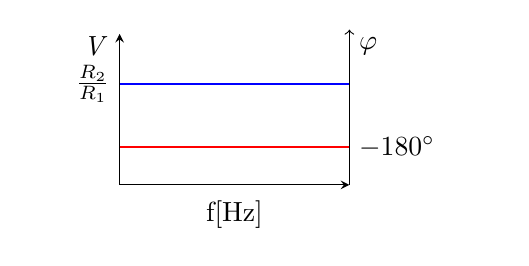
\begin{tikzpicture}[scale=1, transform shape]
    \begin{axis}[
        width=4.5cm, % Breite des Graphen
        height=3.5cm, % Höhe des Graphen
        xmin=0, xmax=10,
        ymin=0, ymax=120,
        axis lines=left,
        axis on top=true,
        domain=0:10,
        xtick=\empty,
        ytick=\empty,
        ylabel style={rotate=270, anchor=east, yshift=0.8cm},
         ylabel={\it V},
        xlabel={f[Hz]},
        clip mode=individual % Verhindert das Abschneiden von Elementen
        ]
        \path[draw=none] (axis cs:-4, 0) rectangle (axis cs:16.6,120);
    
        \addplot+[mark=none, thick, blue] coordinates {(0,80) (10,80)};
        % Adding the left-side label
        \node[anchor=east] at (axis cs:0,80) {$\frac{R_2}{R_1}$};
    \end{axis}
    \begin{axis}[
        width=4.5cm, % Breite des Graphen
        height=3.5cm, % Höhe des Graphen
        xmin=0, xmax=10,
        ymin=-180, ymax=180,
        axis y line*=right,
        axis x line=none,
        ytick=\empty,
        ylabel={$\varphi$},
        ylabel style={rotate=270, anchor=west, yshift=0.8cm},
        clip mode=individual, % Verhindert das Abschneiden von Elementen
        after end axis/.code={
            \draw[->] (axis cs:10,180) -- (axis cs:10,190);
        }
        ]
        \addplot+[mark=none, thick, red] coordinates {(0,-90) (10,-90)};
        \node[anchor=west] at (axis cs:10,-90) {$-180^\circ$};
    \end{axis}
    \end{tikzpicture}
\end{center}
\vspace{1ex}
\[
    U_{\textnormal{A}} = \frac{R_2}{R_1} U_{\textnormal{E}}
\]
    &
    \textbf{Invertierender Verstärker}
\begin{itemize}
    \item -180$^\circ$ Phasenverschiebung zwischen Ein- zu Ausgang
    \item $R_1$ bestimmt den Eingangswiderstand
    \item Niederohmiger Ausgangs-\linebreak widerstand
    \item Anwendungen: \linebreak z.B. Aktiver Spannungsteiler zum Messen hoher Spannungen, wenn $R_1 > R_2$
\end{itemize}
\\ % Zweite Zeile
    \hline
    \centering
    \begin{circuitikz}[scale=0.7, transform shape]
    \ctikzset{
          resistors/scale=0.8,              
          tripoles/en amp/height=1.4, % Höhe des OPV             
          tripoles/en amp/width=1.4,   % Breite des OPV
         tripoles/en amp/input height=0.45
     }
     \draw
     (0,0) node[en amp] (opamp) {}
     (opamp.-)  to[short, o-] ++(0,0) node[left] {$U_{E-}$}
      (opamp.+) to[short, o-] ++(0,0) node[left] {$U_{E+}$}
     (opamp.out) to[short, -o] ++(0,0) node[right] {$U_{A}$};
 \end{circuitikz}
    & 
    \begin{center}
               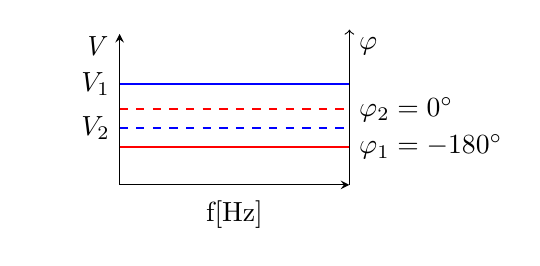
\begin{tikzpicture}[scale=1, transform shape]
    \begin{axis}[
        width=4.5cm, % Breite des Graphen
        height=3.5cm, % Höhe des Graphen
        xmin=0, xmax=10,
        ymin=0, ymax=120,
        axis lines=left,
        axis on top=true,
        domain=0:10,
        xtick=\empty,
        ytick=\empty,
        ylabel style={rotate=270, anchor=east, yshift=0.8cm},
         ylabel={\it V},
        xlabel={f[Hz]},
        clip mode=individual % Verhindert das Abschneiden von Elementen
        ]
        \path[draw=none] (axis cs:-4, 0) rectangle (axis cs:16.6,120);

        \addplot+[mark=none, thick, blue] coordinates {(0,80) (10,80)};
        \addplot+[mark=none, thick, blue, dashed] coordinates {(0,45) (10,45)};
        % Adding the left-side label
        \node[anchor=east] at (axis cs:0,80) {$V_1$};
        \node[anchor=east] at (axis cs:0,45) {$V_2$};
    \end{axis}
    \begin{axis}[
        width=4.5cm, % Breite des Graphen
        height=3.5cm, % Höhe des Graphen
        xmin=0, xmax=10,
        ymin=-180, ymax=180,
        axis y line*=right,
        axis x line=none,
        ytick=\empty,
        ylabel={$\varphi$},
        ylabel style={rotate=270, anchor=west, yshift=0.8cm},
        clip mode=individual, % Verhindert das Abschneiden von Elementen
        after end axis/.code={
            \draw[->] (axis cs:10,180) -- (axis cs:10,190);
        }
        ]
        \addplot+[mark=none, thick, red, dashed] coordinates {(0,0) (10,0)};
        \addplot+[mark=none, thick, red] coordinates {(0,-90) (10,-90)};
        \node[anchor=west] at (axis cs:10,0) {$\varphi_2 = 0^\circ$};
        \node[anchor=west] at (axis cs:10,-90) {$\varphi_1 = -180^\circ$};
    \end{axis}
    \end{tikzpicture}
\[
V_1: U_{\textnormal{E+}} > U_{\textnormal{E-}} \Rightarrow U_{\textnormal{A}} \approx +U_{\textnormal{B}}
\]
\[
V_2: U_{\textnormal{E+}} < U_{\textnormal{E-}} \Rightarrow U_{\textnormal{A}} \approx -U_{\textnormal{B}}
\]
\end{center}
    &\textbf{Komparator}\newline
    Einsatz in Zweipunktreglern und Analog-Digital-Wandlern
\\ % Dritte Zeile
    \hline

    

\centering
\begin{circuitikz}[scale=0.7, transform shape]
    \ctikzset{
        resistors/scale=0.8,              
        tripoles/en amp/height=1.4, % Höhe des OPV             
        tripoles/en amp/width=1.4,   % Breite des OPV
        tripoles/en amp/input height=0.45
    }
    \draw
    (0,0) node[en amp] (opamp) {}
    % R2 mit korrigiertem Strompfeil
    (opamp.-) -- ++(-0.4,0) node[circ] {} to[R, l_=$R_2$] ++(-1.5,0) node[ocirc] (R2left) {}
    % R1 mit korrigiertem Strompfeil
    (opamp.-) -- ++(-0.4,0) --++(0,1) to[R, l_=$R_1$] ++(-1.5,0) node[ocirc] (R1left) {}
    % Erdung
    (opamp.+) -- ++(0,0) node[ground] {}
    % Ausgang
    (opamp.out) to[short, *-o] ++(0,0) node[right] {$U_{A}$}
    % R3 mit Strompfeil
    (opamp.out) -- ++(0,1.5) to[R, l_=$R_3$] ++(-2,0) -- ++(0,-1.05) node[circ] {}
    % Spannungen U_E1 und U_E2 an den Knoten links von R1 und R2
    (R1left) node[left] {$U_{E1}$}
    (R2left) node[left] {$U_{E2}$};
\end{circuitikz}

    &
    \begin{center}
    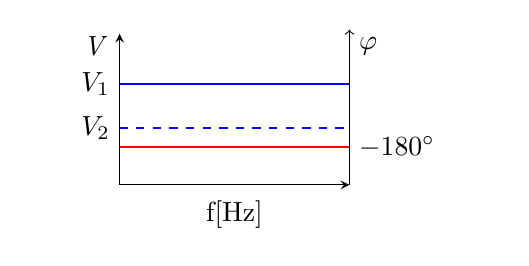
\begin{tikzpicture}[scale=1, transform shape]
    \begin{axis}[
        width=4.5cm, % Breite des Graphen
        height=3.5cm, % Höhe des Graphen
        xmin=0, xmax=10,
        ymin=0, ymax=120,
        axis lines=left,
        axis on top=true,
        domain=0:10,
        xtick=\empty,
        ytick=\empty,
        ylabel style={rotate=270, anchor=east, yshift=0.8cm},
         ylabel={\it V},
        xlabel={f[Hz]},
        clip mode=individual % Verhindert das Abschneiden von Elementen
        ]
        \addplot+[mark=none, thick, blue] coordinates {(0,80) (10,80)};
        \addplot+[mark=none, thick, blue, dashed] coordinates {(0,45) (10,45)};
    
        % Adding the left-side label
        \node[anchor=east] at (axis cs:0,80) {$V_1$};
        \node[anchor=east] at (axis cs:0,45) {$V_2$};
    \end{axis}
    \begin{axis}[
        width=4.5cm, % Breite des Graphen
        height=3.5cm, % Höhe des Graphen
        xmin=0, xmax=10,
        ymin=-180, ymax=180,
        axis y line*=right,
        axis x line=none,
        ytick=\empty,
        ylabel={$\varphi$},
        ylabel style={rotate=270, anchor=west, yshift=0.8cm},
        clip mode=individual, % Verhindert das Abschneiden von Elementen
        after end axis/.code={
            \draw[->] (axis cs:10,180) -- (axis cs:10,190);
        }
        ]
        \path[draw=none] (axis cs:-4, 0) rectangle (axis cs:16.6,120);
        \addplot+[mark=none, thick, red] coordinates {(0,-90) (10,-90)};
        \node[anchor=west] at (axis cs:10,-90) {$-180^\circ$};
    \end{axis}
    \end{tikzpicture}
\end{center}
\vspace{1ex}
\[
\begin{aligned}
    U_{\textnormal{A}} = \underbrace{\frac{R_3} {R_1}}_{V_1} \cdot U_{\textnormal{E1}} + \underbrace{\frac{R_3} {R_2}}_{V_2} \cdot U_{\textnormal{E2}}
\end{aligned}
\]
    & 
    \textbf{Summierer}\newline
    Der Summierer basiert auf dem invertierenden Verstärker und findet Verwendung in Analogrechnern und beim Mischen von Spannungssignalen
    \\ % Vierte Zeile
    \hline
    
    \end{tabular}
\end{table}


\newpage












\begin{table}[ht]
    \begin{tabular}{|m{0.23\textwidth}|m{0.44\textwidth}|m{0.33\textwidth}|}
     \hline 
    Schaltung & Frequenzgang und Gleichung & Erläuterung und Eigenschaften \\ % Neue Zeile mit Text
    \hline
    \begin{circuitikz}[scale=0.7, transform shape]
    \ctikzset{
          resistors/scale=0.8,              
          tripoles/en amp/height=1.4, % Höhe des OPV             
          tripoles/en amp/width=1.4,   % Breite des OPV
         tripoles/en amp/input height=0.45
     }
     \draw
     (0,0) node[en amp] (opamp) {}
     (opamp.-) to[R, l_=$R_1$, o-] ++(-1.2,0) to[short, o-] ++(0,0) node[left] {$U_{E1}$}
     (opamp.+) node[circ] {} to[R,  l_=$R_4$] ++(0,-1.5) node[ground] {}
     (opamp.-) node[circ] {} -- ++(0,1) to[R, l=$R_2$] ++(1.9,0) -| (opamp.out)
     (opamp.out) to[short, *-o] ++(0.2,0) node[right] {$U_{A}$}
     (opamp.+) to[R, l_=$R_3$, *-] ++(-1.2,0) to[short, o-] ++(0,0) node[left] {$U_{E2}$};
 \end{circuitikz}
      &
      \begin{center}
      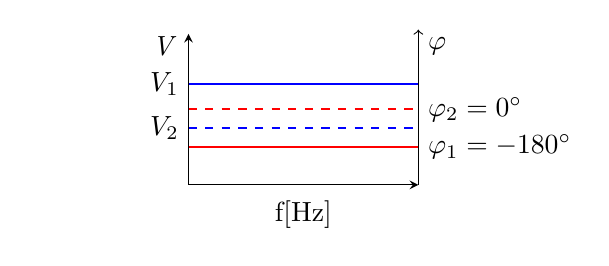
\begin{tikzpicture}[scale=1, transform shape]
    \begin{axis}[
        width=4.5cm, % Breite des Graphen
        height=3.5cm, % Höhe des Graphen
        xmin=0, xmax=10,
        ymin=0, ymax=120,
        axis lines=left,
        axis on top=true,
        domain=0:10,
        xtick=\empty,
        ytick=\empty,
        ylabel style={rotate=270, anchor=east, yshift=0.8cm},
         ylabel={\it V},
        xlabel={f[Hz]},
        clip mode=individual % Verhindert das Abschneiden von Elementen
        ]
        \addplot+[mark=none, thick, blue] coordinates {(0,80) (10,80)};
        \addplot+[mark=none, thick, blue, dashed] coordinates {(0,45) (10,45)};
        % Adding the left-side label
        \node[anchor=east] at (axis cs:0,80) {$V_1$};
        \node[anchor=east] at (axis cs:0,45) {$V_2$};
    \end{axis}
    \begin{axis}[
        width=4.5cm, % Breite des Graphen
        height=3.5cm, % Höhe des Graphen
        xmin=0, xmax=10,
        ymin=-180, ymax=180,
        axis y line*=right,
        axis x line=none,
        ytick=\empty,
        ylabel={$\varphi$},
        ylabel style={rotate=270, anchor=west, yshift=0.8cm},
        clip mode=individual, % Verhindert das Abschneiden von Elementen
        after end axis/.code={
            \draw[->] (axis cs:10,180) -- (axis cs:10,190);
        }
        ]
        \addplot+[mark=none, thick, red, dashed] coordinates {(0,0) (10,0)};
        \addplot+[mark=none, thick, red] coordinates {(0,-90) (10,-90)};
        \node[anchor=west] at (axis cs:10,0) {$\varphi_2 = 0^\circ$};
        \node[anchor=west] at (axis cs:10,-90) {$\varphi_1 = -180^\circ$};
   
   
        \path[draw=none] (axis cs:-7, 0) rectangle (axis cs:16.6,120);
   
   
   
   
    \end{axis}
    \end{tikzpicture}
 \end{center}
 \vspace{1ex}
 \[
 \begin{aligned}
    {U_A} = {U_{{\textnormal{E2}}}} \cdot \underbrace{ \frac{R_1 + R_2}{R_1} \cdot \frac{R_4}{R_3 + R_4}}_{V_2} - U_{\textnormal{E1}} \cdot \underbrace{\frac{R_2}{R_1}}_{V_1}
\end{aligned}
 \]
     &
     \textbf{Subtrahierer}\newline
     Wenn alle Widerstände gleich groß sind, wird die Differenz der Signale $U_{E1}$ und $U_{E2}$ gebildet, weswegen diese Schaltung als Differenzverstärker bezeichnet wird
 \\ % Fünfte Zeile
     \hline

    \begin{circuitikz}[scale=0.7, transform shape]
    \ctikzset{
          resistors/scale=0.8,              
          tripoles/en amp/height=1.4, % Höhe des OPV             
          tripoles/en amp/width=1.4,   % Breite des OPV
         capacitors/scale=0.5,
         tripoles/en amp/input height=0.45
     }
     \vspace{1ex}
     \draw (2,0) node[en amp] (opamp) {}
     (opamp.+) --++ (-0.5,0) node[ground] {} 
     (opamp.out) --++ (0.2,0) node[ocirc, label=right:$U_A$] {}
     (opamp.-) -- ++(0, 0) to[R, l_=$R_1$] ++(-1.2, 0) node[ocirc, label=left:$U_E$] {}
     
     (opamp.out) node[circ] {} -- ++(0,1.5) to[C, l_=$C_1$, *-] ++(-1.9,0) node[circ]{}
     (opamp.out) node[circ] {} -- ++(0,2.8) to[R, l_=$R_2$] ++(-1.9,0) -- ++(0, -2.35) node[circ] {};
     \end{circuitikz}
     & 
     \begin{center}
    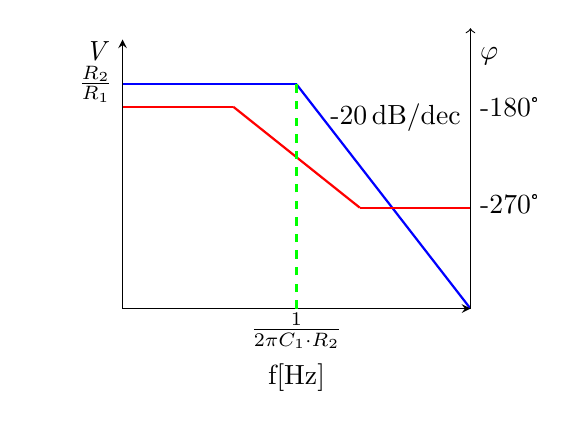
\begin{tikzpicture}[scale=1, transform shape]
    \begin{axis}[
       width=6cm, % Breite des Graphen
       height=5cm, % Höhe des Graphen
        xmin=0, xmax=11,
        ymin=0, ymax=1.2,
        axis lines=center,
        axis on top=true,
        domain=0:10,
        xtick=\empty,
        ytick=\empty,
        ylabel style={xshift=-0.6cm, yshift=0.1cm },
       ylabel={\it V},
       xlabel style={yshift=-0.4cm },
        xlabel={f[Hz]},
        clip mode=individual, % Verhindert das Abschneiden von Elementen
        xlabel style={at={(axis description cs:0.5,-0.05)},anchor=north}
        ]

        \path[draw=none] (axis cs:-3, 0) rectangle (axis cs:13,1);



        \addplot+[mark=none, thick, blue] coordinates {(0,1) (5.5,1)};
        \addplot+[mark=none, thick, blue] coordinates {(5.5,1) (11,0)};
        \node[anchor=east] at (axis cs:0,1) {$\frac{R_2}{R_1}$};
       \node[anchor=east] at (axis cs:11,0.85) {-20\,\text{dB/dec}};
    \end{axis}
    
    \begin{axis}[
       width=6cm, % Breite des Graphen
       height=5cm, % Höhe des Graphen
       xmin=0, xmax=11,
       ymin=0, ymax=240, 
       axis y line*=right,
       axis x line=none,
       ylabel={$\varphi$},
       ylabel style={rotate=270, anchor=west, yshift=1.5cm},
       xtick=\empty,
       ytick=\empty,
       clip mode=individual, % Verhindert das Abschneiden von Elementen
       after end axis/.code={
           \draw[->] (axis cs:11,240) -- (axis cs:11,250);
       }
        ]
        \addplot+[mark=none, thick, red] coordinates {(0,180) (3.5,180)};
        \addplot+[mark=none, thick, red] coordinates {(3.5,180) (7.5,90)};
        \addplot+[mark=none, thick, red] coordinates {(7.5,90) (11,90)};
        \addplot+[mark=none,dashed, thick, green] coordinates {(5.5,0) (5.5,200)};
        \node[] at (axis cs:5.5,-20) {$\frac{1}{2 \pi C_1 \cdot R_2}$};
        \node[anchor=west] at (axis cs:11,180) {-180°};
        \node[anchor=west] at (axis cs:11,93) {-270°};
    \end{axis}
    \end{tikzpicture}
     \[
     U_A(t) = - \frac{R_2}{R_1} U_{\textnormal{E}}(t) - \int_0^t \frac{U_{\textnormal{E}}(t)}{R_1 C_1} \, dt
     \]
     \end{center} 
     &
    \textbf{Integrierer/Integrator}\newline
    \begin{itemize}
        \item Nimmt eine Integration des Eingangssignals vor
        \item Wird als aktives Tiefpassfilter verwendet
    \end{itemize}
      \\ 
      \hline
    \begin{circuitikz}[scale=0.7, transform shape]
    \ctikzset{
          resistors/scale=0.8,              
          tripoles/en amp/height=1.4, % Höhe des OPV             
          tripoles/en amp/width=1.4,   % Breite des OPV
         capacitors/scale=0.5,
         tripoles/en amp/input height=0.45
     }
     \draw (2,0) node[en amp] (opamp) {}
     (opamp.+) --++ (-0.5,0) node[ground] {} 
     (opamp.out) --++ (0.2,0) node[ocirc, label=right:$U_A$] {}
     (opamp.-) -- ++(0, 0) to[C, l_=$C_2$] ++(-0.5, 0) to[R, l_=$R_1$] ++(-1.2,0) node[ocirc, label=left:$U_E$] {}
     (opamp.out) node[circ] {} -- ++(0,1.5) to[C, l_=$C_1$, *-] ++(-1.9,0) node[circ]{}
     (opamp.out) node[circ] {} -- ++(0,2.8) to[R, l_=$R_2$] ++(-1.9,0) -- ++(0, -2.35) node[circ] {};
  
 \end{circuitikz}
    &
    \begin{center}
    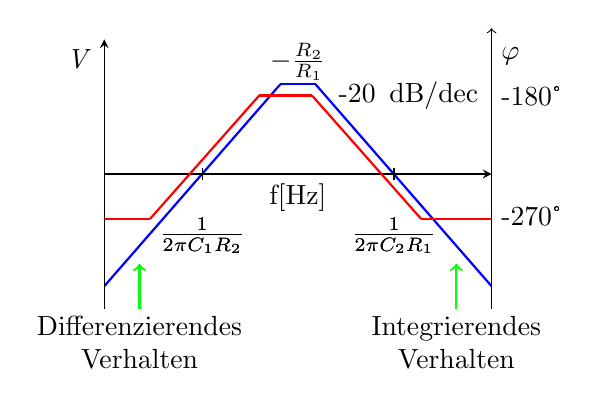
\begin{tikzpicture}[scale=1, transform shape]
    \begin{axis}[
        width=6.5cm, % Breite des Graphen
        height=5cm, % Höhe des Graphen
        xmin=0, xmax=11,
        ymin=-1.2, ymax=1.2,
        axis lines=center,
        axis on top=true,
        domain=0:10,
        clip mode=individual, % Verhindert das Abschneiden von Elementen
        xtick=\empty,
        ytick=\empty,
        ylabel style={xshift=-0.6cm},
        ylabel={\it V},
        xlabel={f[Hz]},
        xlabel style={at={(axis description cs:0.5,0.5)},anchor=north}
        ]
        \path[draw=none] (axis cs:-2, 0) rectangle (axis cs:13,1); \path[draw=none] (axis cs:-2, 0) rectangle (axis cs:13,1);


        \addplot+[mark=none, thick, blue] coordinates {(0,-1) (5,0.8)};
        \addplot+[mark=none, thick, blue] coordinates {(5,0.8) (6,0.8)};
        \addplot+[mark=none, thick, blue] coordinates {(6,0.8) (11,-1)};
        \node[anchor=north] at (axis cs:5.5,1.25) {$-\frac{R_2}{R_1}$};
        \addplot+[only marks, mark=|, black] coordinates {(2.78,0)} node[anchor=south] at (axis cs:2.78,-0.8) {$\frac{1}{2 \pi C_1 R_2}$};
        \addplot+[only marks, mark=|, black] coordinates {(8.23,0)} node[anchor=south] at (axis cs:8.23,-0.8) {$\frac{1}{2\pi C_2 R_1}$};
        \node[anchor=east] at (axis cs:10.9,0.7) {-20\, \text{dB/dec}};
        \addplot+[only marks, mark=|, black] coordinates {(2.78,0)} node[anchor=south] at (axis cs:2.78,-0.8) {$\frac{1}{2 \pi C_1 R_2}$};
        \addplot+[only marks, mark=|, black] coordinates {(8.23,0)} node[anchor=south] at (axis cs:8.23,-0.8) {$\frac{1}{2\pi C_2 R_1}$};
        \draw[->, thick, green] (axis cs:1,-1.2) -- (axis cs:1,-0.8);
        \node[align=center, black] at (axis cs:1,-1.5) {Differenzierendes\\ Verhalten};
        
        \draw[->, thick, green] (axis cs:10,-1.2) -- (axis cs:10,-0.8);
        \node[align=center, black] at (axis cs:10,-1.5) {Integrierendes\\ Verhalten};
        
    \end{axis}
    
    \begin{axis}[
        width=6.5cm, % Breite des Graphen
        height=5cm, % Höhe des Graphen
        xmin=0, xmax=11,
        ymin=0, ymax=240, 
        axis y line*=right,
        axis x line=none,
        ylabel={$\varphi$},
        ylabel style={rotate=270, anchor=west, yshift=1.5cm},
        xtick=\empty,
        ytick=\empty,
        clip mode=individual, % Verhindert das Abschneiden von Elementen
        after end axis/.code={
            \draw[->] (axis cs:11,240) -- (axis cs:11,250);
        }
        ]
        \addplot+[mark=none, thick, red] coordinates {(0,80) (1.3,80)};
        \addplot+[mark=none, thick, red] coordinates {(1.3,80) (4.4,190)};
        \addplot+[mark=none, thick, red] coordinates {(4.4,190) (5.9,190)};
        \addplot+[mark=none, thick, red] coordinates {(5.9,190) (9,80)};
        \addplot+[mark=none, thick, red] coordinates {(9,80) (11,80)};
        \node[anchor=west] at (axis cs:11,82.5) {-270°};
        \node[anchor=west] at (axis cs:11,190) {-180°};
       
    \end{axis}

    
    \end{tikzpicture}
    \begin{multline*}
        U_A = - \frac{R_2}{R_1} U_{\textnormal{E}}(t) \\
        - \int_0^t \frac{1}{R_1 C_1} U_{\textnormal{E}}(t) \, dt 
        - R_2 C_2\frac{dU_{\textnormal{E}}(t)}{dt}
    \end{multline*}
    \end{center} 
    & 
    \textbf{Differenzierer}\newline
    \begin{itemize}
        \item Nimmt eine Integration des Eingangssignals vor
        \item Wird als aktives Hochpassfilter verwendet (zeigt in der Realität meist Bandpassverhalten, wie hier dargestellt)
    \end{itemize}
    \\
    \hline
\end{tabular}
\end{table}






\newpage
    \begin{table}[ht]
        \begin{tabular}{|m{0.285\textwidth}|m{0.395\textwidth}|m{0.33\textwidth}|}
            \hline 
    Schaltung & Frequenzgang und Gleichung & Erläuterung und Eigenschaften \\ % Neue Zeile mit Text
    \hline
    \begin{circuitikz}[scale=0.7, transform shape]
    \ctikzset{
          resistors/scale=0.8,              
          tripoles/en amp/height=1.4, % Höhe des OPV             
          tripoles/en amp/width=1.4,   % Breite des OPV
         diodes/scale=0.8,
         tripoles/en amp/input height=0.45
     }
     \draw
     (0,0) node[en amp] (opamp) {}
     (opamp.-) to[R, l_=$R_1$, *-] ++(-1.2,0) to[short, o-] ++(0,0) node[left] {$U_E$}
     (opamp.+) -- ++(0,0) node[ground] {}
     (opamp.-) |- ++(0,1.5) to[D, l^=$D_1$] ++(2,0) -| (opamp.out)
     (opamp.out) to[short, *-o] ++(0.2,0) node[right] {$U_{A}$};
 \end{circuitikz}
    &
    \begin{center}
    \[
    U_{\textnormal{A}} =-U_{\textnormal{T}}\cdot \ln{\left(\frac{U_{\textnormal{E}}}{R_1\cdot I_S}\right)}
    \]
        \[
            U_{\textnormal{T}} = \frac{k_{\textnormal{B}} \cdot T}{e}
            \]
            
            \(e = \text{Elementarladung}\)
            
            \(k_{\textnormal{B}} = \text{Boltzmannkonstante}\)
            
            \(I_{\textnormal{s}} = \text{Sperrstrom der Diode}\)
    \end{center} 
    & 
    \textbf{Logarithmierer}\newline
    Bildet den natürlichen Logarithmus des Eingangssignals
    \\
    \hline
    \begin{circuitikz}[scale=0.7, transform shape]
    \ctikzset{
          resistors/scale=0.8,              
          tripoles/en amp/height=1.4, % Höhe des OPV            
          tripoles/en amp/width=1.4,   % Breite des OPV
         diodes/scale=0.8,
         tripoles/en amp/input height=0.45
     }
     \draw
     (0,0) node[en amp] (opamp) {}
     (opamp.-) to[D, l_=$D_1$, invert, *-] ++(-1.2,0) to[short, o-] ++(0,0) node[left] {$U_E$}
     (opamp.+) -- ++(0,0) node[ground] {}
     (opamp.-) |- ++(0,1.5) to[R, l^=$R_1$] ++(2,0) -| (opamp.out)
     (opamp.out) to[short, *-o] ++(0.2,0) node[right] {$U_{A}$};
 \end{circuitikz}
    &
    \begin{center}
    \[
    U_{\textnormal{A}} =-R_1\cdot I_{\textnormal{S}} \cdot e^{\frac{U_{\textnormal{E}}}{U_{\textnormal{T}}}}
    \]
    \end{center} 
    & 
    \textbf{Potenzierer}\newline
    Besitzt einen e-funktionalen Zusammenhang zwischen Ein- und Ausgangsspannung
    \\
    \hline
    \begin{circuitikz}[scale=0.6, transform shape]
    \ctikzset{
         resistors/scale=0.8,              
         tripoles/en amp/height=1.4, % Höhe des OPV             
         tripoles/en amp/width=1.4   % Breite des OPV
    }
    \draw 
    % Erster OPV mit input height=-0.45
    (2,-4.5) node[en amp, noinv input down] (opamp1) {}
    (opamp1.+) --++ (-0.5,0) node[ocirc, label=left:$U_{E2}$] (eingang1) {};
    
   \draw (2,0) node[en amp, noinv input up] (opamp2) {}
    (opamp2.+) --++ (-0.5,0) node[ocirc, label=left:$U_{E1}$] (eingang2) {}
    (opamp1.-)  to[R=$R_g$] (opamp2.-);

   % Dritter OPV mit angepasstem Eingangsabstand
    \ctikzset{tripoles/en amp/input height=0.55} % Anpassung nur für diesen OPV
    \draw (6,-2.25) node[en amp] (opamp3) {}
    (opamp3.-) -- ++(-0.5,0) to[R=$R_1$] ++(-1.5,0) to[R=$R_2$] ++(-2,0) node[circ]{}
    (opamp3.+) -- ++(-0.5,0) to[R=$R_3$] ++(-1.5,0) to[R=$R_4$] ++(-2,0) node[circ]{}
    (opamp2.out) -- ++(0,-1.72) node[circ]{}
    (opamp1.out) -- ++(0,1.72) node[circ]{}
    (opamp3.out) node[circ, label=below:{$U_A$}]{} -- ++(0, 2) to[R=$R_5$] ++(-2,0) -- ++(0, -1.45)node[circ]{};

\end{circuitikz}
     &
         \begin{center}
   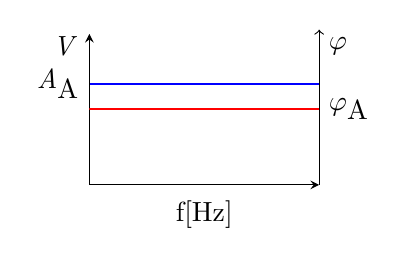
\begin{tikzpicture}[scale=1, transform shape]
    \begin{axis}[
        width=4.5cm, % Breite des Graphen
        height=3.5cm, % Höhe des Graphen
        xmin=0, xmax=10,
        ymin=0, ymax=120,
        axis lines=left,
        axis on top=true,
        domain=0:10,
        xtick=\empty,
        ytick=\empty,
        ylabel style={rotate=270, anchor=east, yshift=0.8cm}, % Position der Beschriftung oben links, horizontal
         ylabel={\it V}, % Hier die gewünschte Beschriftung einfügen
        xlabel={f[Hz]},
        clip mode=individual % Verhindert das Abschneiden von Elementen
        ]
        \addplot+[mark=none, thick, blue] coordinates {(0,80) (10,80)};
        % Adding the left-side label
        \node[anchor=east] at (axis cs:0,80) {$\mathit{A}_{\textnormal{A}}$};
    \end{axis}
    \begin{axis}[
        width=4.5cm, % Breite des Graphen
        height=3.5cm, % Höhe des Graphen
        xmin=0, xmax=10,
        ymin=-180, ymax=180,
        axis y line*=right,
        axis x line=none,
        ytick=\empty,
        ylabel={$\varphi$},
        ylabel style={rotate=270, anchor=west, yshift=0.8cm},
        clip mode=individual, % Verhindert das Abschneiden von Elementen
        after end axis/.code={
            \draw[->] (axis cs:10,180) -- (axis cs:10,190);
        }
        ]
        \addplot+[mark=none, thick, red] coordinates {(0,0) (10,0)};
        \node[anchor=west] at (axis cs:10,0) {$\varphi_{\textnormal{A}}$};
    \end{axis}
    \end{tikzpicture}
\end{center}

\vspace{1ex}
\[
\mathit{a_i} : \text{Amplitude Eingangsspannung i}
\]
\[
\mathit{\varphi_i} : \text{Phase Eingangsspannung i}
\]
\[
\mathit{A}_{A} = \sqrt{a_1^2 + a_2^2 + 2a_1a_2 \cos(\varphi_1 - \varphi_2)}
\]
\[
\mathit{\tan}(\varphi_A) = \frac{a_1 \mathit{\sin}(\varphi_1) + a_2 \mathit{\sin}(\varphi_2)}{a_1 \mathit{\cos}(\varphi_1) + a_2 \mathit{\cos}(\varphi_2)}
\]
\[
    \text{Wenn} : R_2 = R_4 = R
\]
\[
    U_{\textnormal{A}} = (1+ \frac{2R} {R_{\textnormal{g}}}) \cdot \frac{R_3} {R_2} (U_{\textnormal{E2}}-U_{\textnormal{E1}})
\]
     & 
     \textbf{Instrumentenverstärker}\newline
    Differenzverstärker mit hoher Eingangsimpedanz und hoher Gleichtaktunterdrückung  

    \\
    \hline
    \end{tabular}
\end{table}

